\chapter{Eletricidade Cerebral}



\section{Correntes Elétricas}
Quando existe diferença de potencial elétrico entre um material condutor, 
ocorre um fluxo de cargas ao qual se da o nome de \textbf{corrente elétrica} (Creder, 1989).
A intensidade do fluxo é medida em ampère (A) e determinada pela quantiadade de partículas que atravessam o seguimento
do condutor pelo tempo. As correntes podem ser contínuas ou alternadas, a depender se o sentido da corrente varia ou não. Enquanto a corrente contínua 
é composta de polos (positivo e negativo), a alternada é composta de fases (Bhargava e Kulshreshtha, 1983). O calculo de corrente elétrica é 
dado pela seguinte equação:

\begin{equation}
    I = \frac{\Delta Q }{\Delta T},
\end{equation}

onde $\Delta Q$ é a quantidade de particulas que passam em um seguimento do condutor e $\Delta T$ indica o tempo. 

\section{Neurônios}
Os neurônios são células responsáveis pela condução de impulsos nervosos e se comportam como um “cabo eletrificado” - analogia
levantada a respeito da condução de impulsos elétricos, como apresentado no clássico estudo de Hodgkin e Huxley (1952), 
que teve como resultado uma modelagem dos potenciais de ação emitidos pelas células 
nervosas através de equações diferenciais não-lineares, como a descrita na equação 2.1 
para o calculo da corrente elétrica da membrana celular. 

Existem aproximadamente 86 bilhões de neurônios no cérebro (Caire et al., 2022). Os neurônios comunicam-se uns com os outros através das \textbf{sinapses}, onde ocorre a transmissão dos impulsos nervosos. 
É possível distinguir três partes anatomicas no neurônio: o corpo celular, o axônio e os dendrito (figura 2.1).

%https://www.ncbi.nlm.nih.gov/books/NBK441977/
\begin{figure}[h]
    \centering
    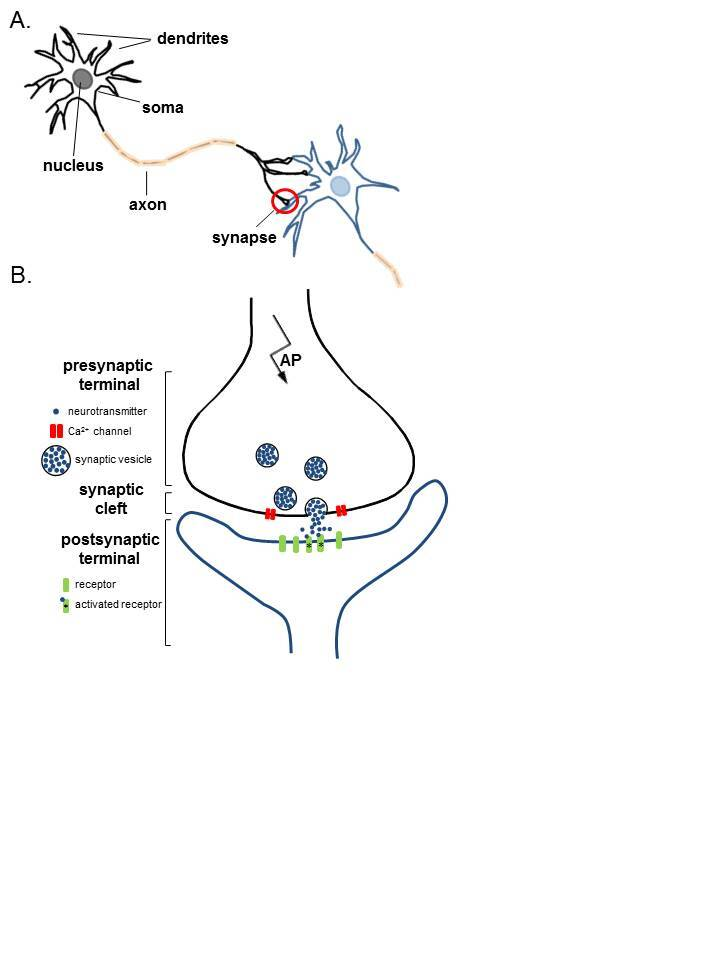
\includegraphics[width=100mm]{Aubrey__Synapse__Figure__1.jpeg}
    \caption[Impulsos nervosos conduzidos em neurônios]{Impulsos nervosos conduzidos em neurônios. Fonte: Ludwig et al. (2021).}.\label{fig:potencial}
    \end{figure}


\subsection{Impulsos Nervosos e Potencial de Ação}
Para passar informações, os neurônios geram \textbf{impulsos nervosos}, ou alterações no potencial elétrico de sua membrana. Este sinal elétrico
ocorre quando o estímulo recebido pelo neurônio ultrapassa um limiar de ativação, que desencadeia uma série de respostas celulares. A célula pode 
estar em repouso (com valor do interior celular em cerca de -70mV), passando por despolarização (quando ocorre um fluxo de cargas elétricas que faz com 
que o meio intracelular passe a ser positivo em relação ao meio extracelular), e em repolarização, quando a célula está retornando ao potencial de repouso,
como representado na figura 2.1. 

\begin{figure}[h]
    \centering
    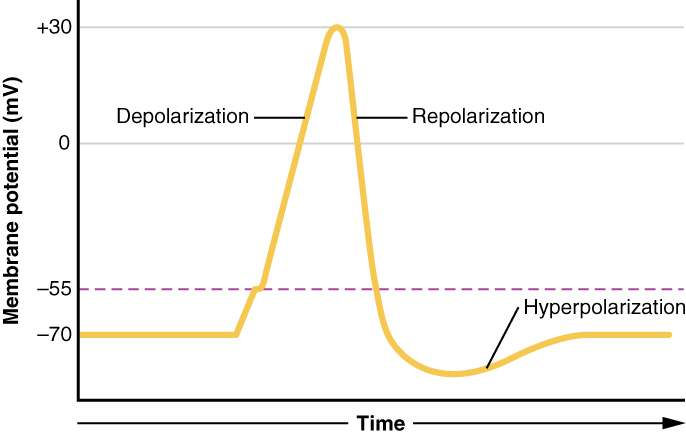
\includegraphics[width=100mm]{Action_Potential.jpeg}
    \caption[Impulsos nervosos conduzidos em neurônios]{Impulsos nervosos conduzidos em neurônios. Fonte: Chen e Lui (2021).}.\label{fig:potencial}
    \end{figure}

\section{Eletroencefalograma}
O conjunto de impulsos nervosos de grupos de neurônios geram campos magnéticos
 que podem ser captados por eletrodos colocados sobre a cabeça humana (Kandel, 2000). 
 Estes campos magnéticos foram primeiro registrados de coletas em humanos aproximadamente em 1929,
  em um experimento conduzido pelo psiquiatra alemão Hans Berger (İnce et al., 2021) – figura 2.2. 
  \begin{figure}[h]
    \centering
    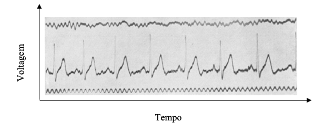
\includegraphics[width=100mm]{serie_temporal_EEG}
    \caption[]{Primeiro EEG registrado em humanos, resultado do trabalho do psiquiatra Hans Berger. Fonte: Ince et al. (2021).} 
    \end{figure}


  Estes registros são o resultado dos potenciais de ação emitidos pelas células nervosas abaixo do eletrodo, 
  e permitem uma boa resolução temporal do comportamento nervoso (podendo atingir precisão de milissegundos), 
  mas em geral não permitem uma boa resolução espacial (como identificar a localização espacial do grupo celular responsável pela variação de voltagem observada). 



  

    \subsection{Tipos de Eletrodos para Captura de EEG}

    Existem diferentes tipos de eletrodos para a captura de EEG. Um resumo é apresentado na tabela 2.1. É notável também que com o desenvolvimento da capacidade computacional, novos recursos e métodos para a análise destes dados vem sendo benéficos à construção do conhecimento científico, agora também contando com o desenvolvimento de algoritmos de aprendizado de máquina, aprendizado profundo e inteligência artificial. 
  
\subsection{Sistema Internacional 10/20 de Posicionamento de Eletrodos}

A técnica de registro de EEG vem sendo desde então aperfeiçoada e escolhida em investigações 
comportamentais devido a sua natureza não invasiva.
 Um exemplo de aperfeiçoamento foi a criação de um sistema internacional de posicionamentos 
 de eletrodos para a coleta de EEG – o sistema 10/20 (Klem et al., 1999), 
 representado na figura 2.3. 
 O registro capturado nos eletrodos advém de uma 
 diferença de potencial elétrico. Esta diferença pode ser em 
 referência à um eletrodo colocado em uma região externa ao escalpo (como orelha), 
 ou à uma voltagem média comum (Tavares, 2011).




%\subsection{Potenciais Relacionados a Eventos}


